\usetikzlibrary{patterns}
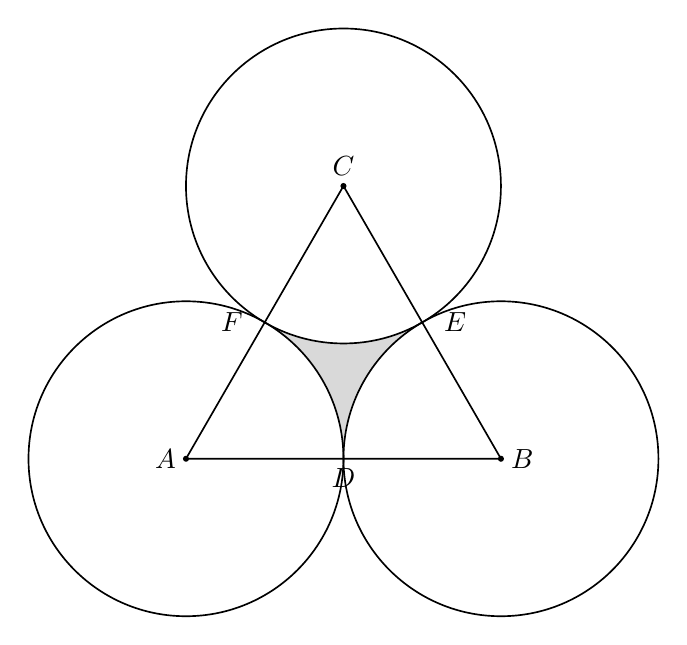
\begin{tikzpicture}[x=1cm,y=1cm,line width=.6pt,font=\normalsize]
\coordinate (A) at (0,0);
\coordinate (B) at (4,0);
\coordinate (C) at (2,3.46410);
\coordinate (D) at (2,0);
\coordinate (E) at (3,1.73205);
\coordinate (F) at (1,1.73205);
\fill[fill=black!15,draw=none] (A)--(B)--(C)--cycle;
\fill[white,draw=none] (A) circle[radius=2cm];
\fill[white,draw=none] (B) circle[radius=2cm];
\fill[white,draw=none] (C) circle[radius=2cm];
\draw (A) circle[radius=2cm];
\draw (B) circle[radius=2cm];
\draw (C) circle[radius=2cm];
\draw (A)--(B)--(C)--cycle;
\fill (A) circle[radius=1.1pt];
\fill (B) circle[radius=1.1pt];
\fill (C) circle[radius=1.1pt];
\node[left] at (A) {$A$};
\node[right] at (B) {$B$};
\node[above] at (C) {$C$};
\node[below] at (D) {$D$};
\node[right,xshift=1.5mm] at (E) {$E$};
\node[left,xshift=-1.5mm] at (F) {$F$};
\end{tikzpicture}
